In this section, we study proportionality on real data taken from the UCI Machine Learning Repository~\cite{UCI}. We consider three qualitatively different data sets used for clustering: Iris, Diabetes, and KDD. For each data set, we only have a single set of points given as input, so we take $\N = \M$ to be the set of all points in the data set. We use the standard Euclidean L2 distance.

\textbf{Iris.} This data set contains information about the petal dimensions of three different species of iris flowers. There are 50 samples of each species.

\textbf{Diabetes.} The Pima Indians Diabetes data set contains information about 768 diabetes patients, recording features like glucose, blood pressure, age and skin thickness. 

\textbf{KDD.} The KDD cup 1999 data set contains information about sequences of TCP packets. Each packet is classified as normal or one of twenty-two types of intrusions. Of these 23 classes, normal, ``neptune'', and ``smurf'' account for 98.3$\%$ of the data. The data set contains 18 million samples; we work with a subsample of 100,000 points.\footnote{We run $k$-means++ on this entire 100,000 point sample. For efficiency, we run our Local Capture algorithm by further sampling 5,000 points uniformly at random to treat as $\N$ and sampling 400 points via the $k$-means++ initialization to treat as $\M$. For the sake of a fair comparison, we generate a different sample of 400 centers using the $k$-means++ initialization that we use to determine the value of $\rho$ we report for both Local Capture and the $k$-means++ algorithm. The $k$-means objective is measured on the original 100,000 points for both algorithms.}%We consider this $98.3\%$ as non-outliers and consider the rest $1.7\%$ as outliers. Note that due to the existence of outliers, we expect to see that \textbf{k-means++} will tend to find more unfair solution in our setting. Due to the scale of this dataset, we run Iterative Block algorithm over a sample of 5000 clients and 400 centers. According to Theorem 3, we know, with high probability, our algorithm will find a solution, which is $\rho$-proportional to the sample and $\rho$-proportional to $(1+\epsilon)$-deviations to the whole data set. 

\subsection{Proportionality and $k$-means Objective Tradeoff}

We compare Greedy Capture (Algorithm~\ref{alg:ball}) and Local Capture (Algorithm~\ref{alg:local}) with the $k$-means++ algorithm (Lloyd's algorithm for $k$-means minimization with the $k$-means++ initialization~\cite{kmeans++}) for a range of values of $k$. For the Iris data set, Local Capture  and $k$-means++ always find an exact proportional solution (Figure~\ref{fig:IrisRho}), and have comparable $k$-means objectives (Figure~\ref{fig:IriskMeans}). The Iris data set is very simple with three natural clusters, and validates the intuition that proportionality and the $k$-means objective are not always opposed.

The Diabetes data set is larger and more complex. As shown in Figure~\ref{fig:DiabetesRho}, $k$-means++ no longer always finds an exact proportional solution. Local Capture always finds a better than 1.01-proportional solution. As shown in Figure~\ref{fig:DiabeteskMeans}, the $k$-means objectives of the solutions are separated, although generally on the same order of magnitude.

\begin{figure*}[t!]
    \centering
    \begin{subfigure}[t]{0.33\linewidth}
        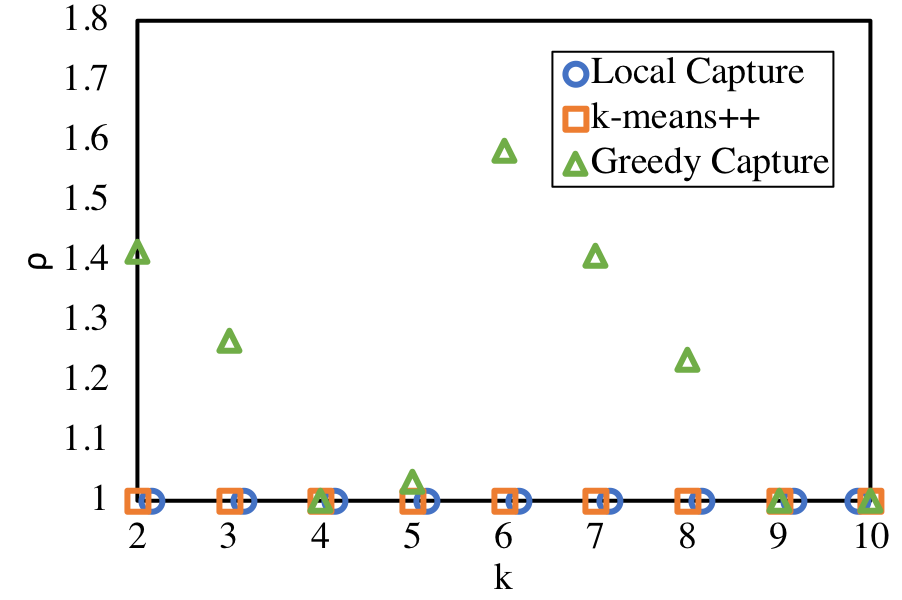
\includegraphics[width=\linewidth]{IrisRho.png}
        \caption{Iris}
        \label{fig:IrisRho}
    \end{subfigure}%
    ~
    \begin{subfigure}[t]{.33\linewidth}
        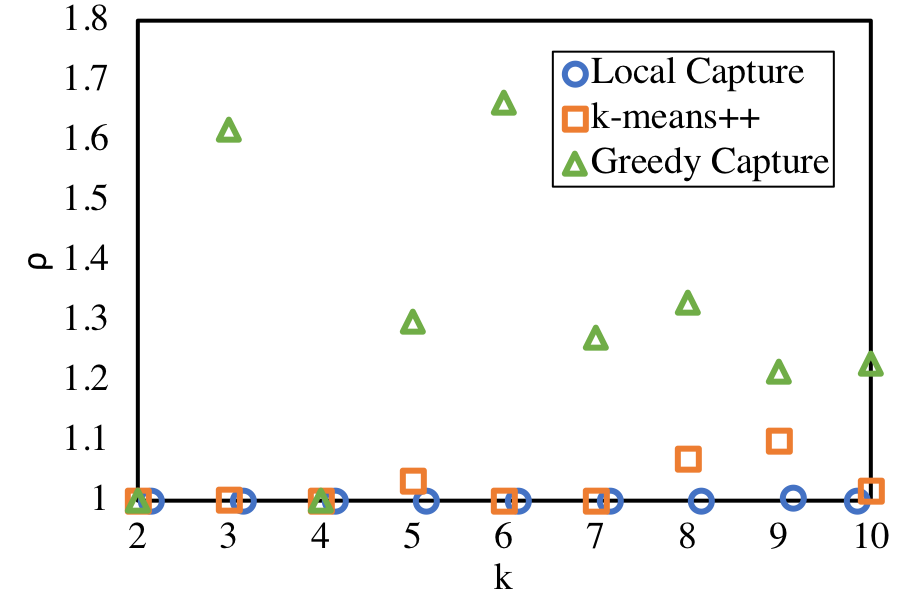
\includegraphics[width=\linewidth]{DiabetesRho.png}
        \caption{Diabetes}
        \label{fig:DiabetesRho}
    \end{subfigure}%
    ~
    	 \begin{subfigure}[t]{.33\linewidth}
        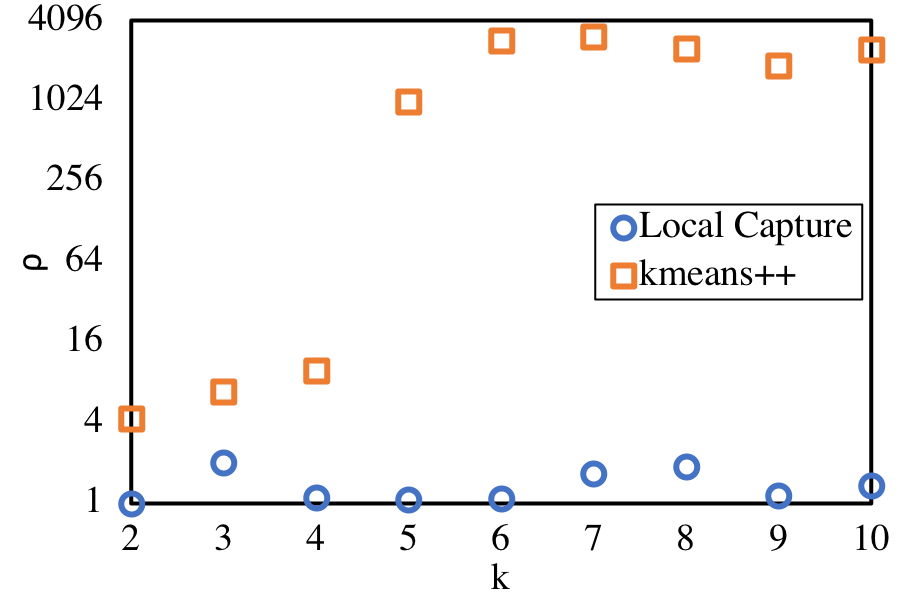
\includegraphics[width=\linewidth]{kddRho.png}
        \caption{KDD, geometric scale}
        \label{fig:kddRho}
    \end{subfigure}%
    \caption{Minimum $\rho$ such that the solution is $\rho$-proportional}.
    \label{fig:Rho}
\end{figure*}
    
\begin{figure*}[t!]
    \centering
    \begin{subfigure}[t]{0.33\linewidth}
        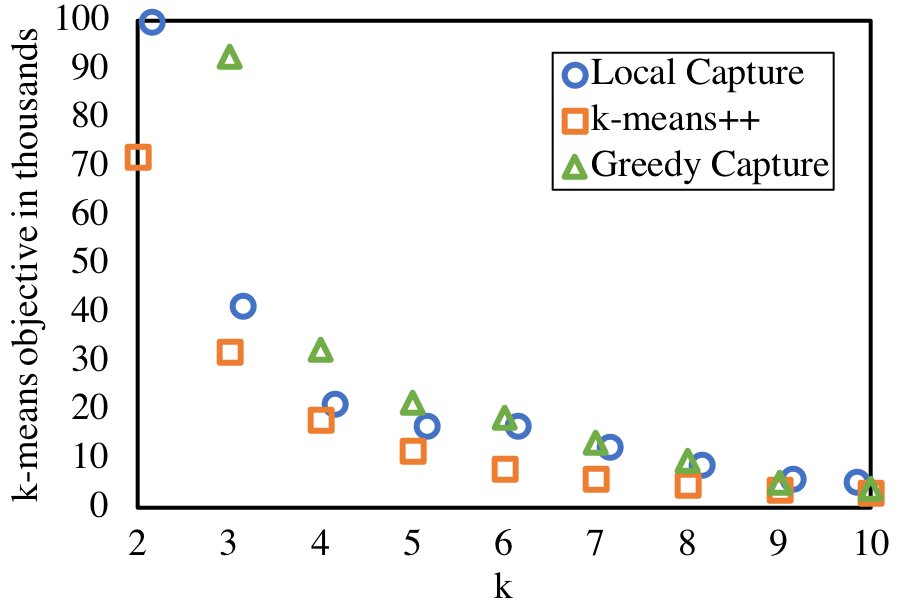
\includegraphics[width=\linewidth]{IriskMeans.png}
        \caption{Iris}
        \label{fig:IriskMeans}
    \end{subfigure}%
    ~
    \begin{subfigure}[t]{0.33\linewidth}
        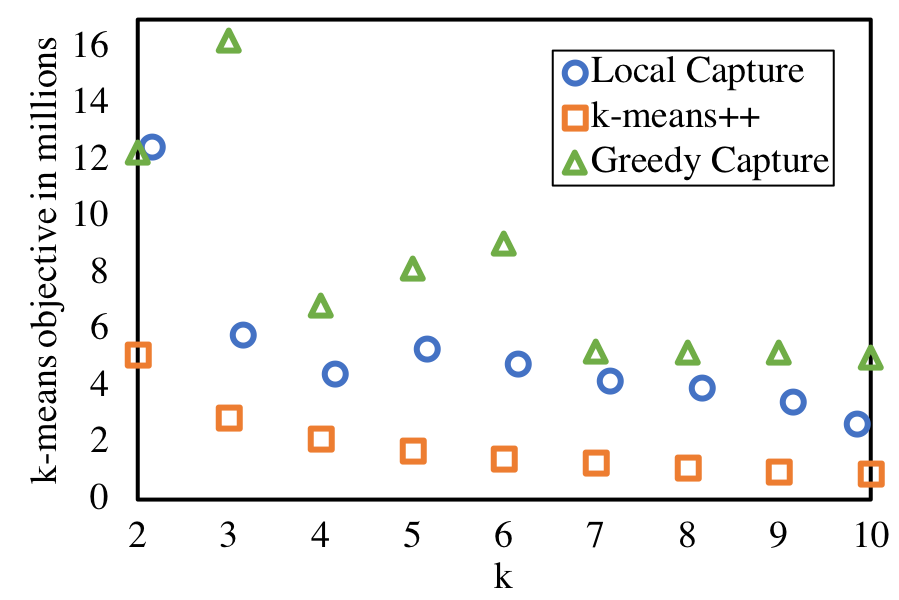
\includegraphics[width=\linewidth]{DiabeteskMeans.png}
        \caption{Diabetes}
        \label{fig:DiabeteskMeans}
    \end{subfigure}%
    ~ 
    \begin{subfigure}[t]{0.33\linewidth}
        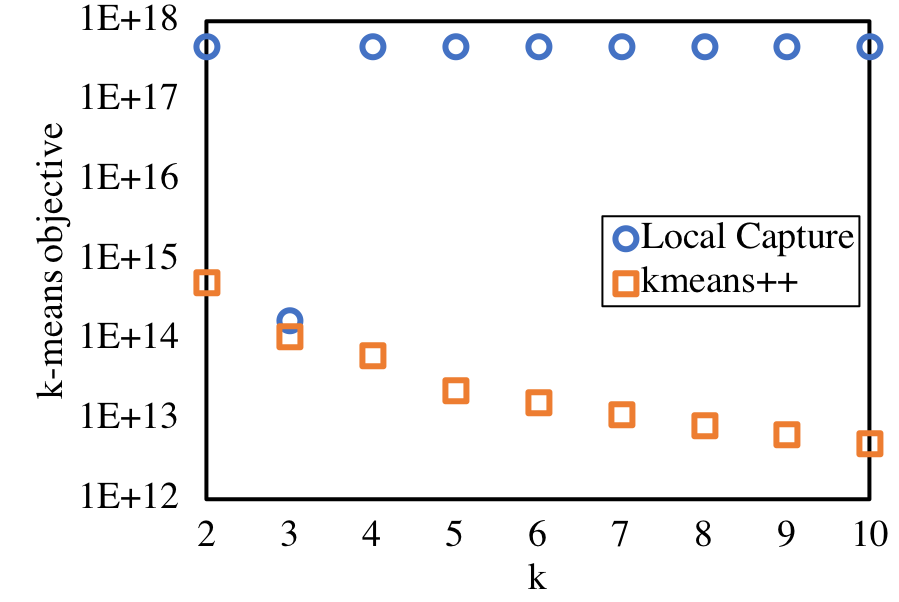
\includegraphics[width=\linewidth]{kddkMeans.png}
        \caption{KDD, geometric scale}
        \label{fig:kddObjective}
    \end{subfigure}
    \caption{$k$-means objective}
\end{figure*}

For the KDD data set, proportionality and the $k$-means object appear to be in conflict. Greedy Capture's performance is comparable to Local Capture on KDD, so we omit it for clarity. In Figures~\ref{fig:kddRho} and~\ref{fig:kddObjective}, note that the gap between $\rho$ and the $k$-means objective for the $k$-means++ and Local Capture algorithms is between three and four orders of magnitude. We suspect this is due to the presence of significant outliers in the KDD data set. This is in keeping with the theoretical impossibility of simultaneously approximating the optima on both objectives, and demonstrates that this tension arises in practice as well as theory.


%$k$-means++ algorithm only finds a roughly 4,000-proportional clustering. On the other hand, Local Capture is still consistently able to find a roughly 2-proportional clustering or better. There is a similarly dramatic difference of between three and five orders of magnitude in the $k$-means objectives achieved by the algorithms, as seen in Figure~\ref{fig:kddObjective}. This behavior appears to be due to the presence of significant outliers in the KDD data set. This is in keeping with the theoretical impossibility of simultaneously approximating the optima on both objectives, and demonstrates that this tension arises in practice as well as theory. %From an applied perspective then, the data analyst cannot assume that standard clustering algorithms will necessarily produce approximately proportional clusterings.   

\subsection{Proportionality and Low $k$-means Objective}
Note that if one is allowed to use $2k$ centers when $k$ is given as input, one can trivially achieve the proportionality of Local Capture and the $k$-means objective of the $k$-means++ algorithm by taking the union of the two solutions. Thinking in this way leads to a different way of quantifying the tradeoff between proportionality and the $k$-means objective: Given an approximately proportional solution, how many \textit{extra} centers are necessary to get comparable $k$-means objective as the $k$-means++ algorithm? For a given data set, the answer is a value between 0 and $k$, where larger numbers indicate more incompatibility, and lower numbers indicate less incompatibility.  

To answer this question, we compute the union of centers found by Local Capture and the $k$-means++ algorithm. We then greedily remove centers as long as doing so does not increase the minimum $\rho$ such that the solution is $\rho$-proportional (defined on $k$, not $2k$) by more than a multiplicative factor of $\alpha$, and does not increase the $k$-means objective by more than a multiplicative factor $\beta$.  

%On a data set like KDD, a natural question is whether we can find a solution that does well on proportionality and the $k$-means objective by relaxing some other feature of the problem. In particular, we consider relaxing the constraint that we must use at most $k$ centers. Toward that end, consider the following solution with $2k$ centers: $k$ from Local Capture and $k$ from the $k$-means++ algorithm. Call this set of $2k$ centers $X$. Let $\rho^* = \rho(X) = \min_{\rho \geq 1}$ such that $X$ is a $\rho$-proportional solution (for the original value $k$), and let $\kappa^* = \kappa(X) = \sum_{i \in N} \left( D_i(X) \right)^2$ (i.e., the $k$-means objective). Clearly, $\rho^*$ and $\kappa^*$ will be at most the values obtained by running Local Capture and $k$-means++ respectively, since we took the union of the two solutions. Therefore, we can achieve small values on both measures with $k$ extra centers. We now present a heuristic that greedily removes unwanted centers while preserving both measures approximately.

%Fix two small constants $\alpha, \beta \ge 1$. The heuristic attempts to remove centers as long as the removals do not worsen the approximation to proportionality by more than a multiplicative factor $\alpha$ or the $k$-means objective by more than a multiplicative factor $\beta$.  In other words, while there is a center $y \in X$ such that $\rho(X \setminus \{y\}) \le \alpha \rho^*$ and $\kappa(X \setminus \{y\}) \le \beta \kappa^*$, remove $y$ from the set $X$. In the end, we obtain a solution $X$ whose $\rho(X) \le \alpha \rho^*$ and $\kappa(X) \le \beta \kappa^*$.

On the KDD dataset, we set $\alpha = 1.2$ and $\beta = 1.5$, so the proportionality of the result is within 1.2 of Local Capture in Figure~\ref{fig:kddRho}, and the $k$-means objective is within 1.5 of $k$-means++ in Figure~\ref{fig:kddObjective}.  We observe that this heuristic uses at most $3$ extra centers for any $k \le 10$. So while there is real tension between proportionality and the $k$-means objective, this tension is still not maximal. In the worst case, one might need to add $k$ centers to a proportional solution to compete with the $k$-means objective of the $k$-means++ algorithm, but in practice we find that we need at most $3$ for $k \le 10$. 

\iffalse
Let $\rho(X) = \min_{\rho \geq 1}$ such that $X$ is a $\rho$-proportional solution, and let $\kappa(X) = \sum_{i \in N} \left( D_i(X) \right)^2$ (i.e., the $k$-means objective).

Figure~\ref{fig:hybridHeuristic} shows that on the KDD data set, the heuristic needs between 0 and 3 extra centers to simultaneously approximate Local Capture and $k$-means++. We set $\alpha = 1.2$ and $\beta = 1.5$, so the proportionality of the result is within 1.2 of Local Capture in Figure~\ref{fig:kddRho}, and the $k$-means objective is within 1.5 of $k$-means++ in Figure~\ref{fig:kddObjective}. 

\begin{algorithm}
\begin{algorithmic}[1]
\caption{Hybrid Heuristic}
\label{alg:heuristic}
	\INPUT $\alpha, \beta$
	\STATE Run Algorithm~\ref{alg:local} to find $k$ centers $X$
	\STATE Run K-Means++ Algorithm to find $k$ centers $Y$
	\STATE $Z = X \cup Y$
	\REPEAT
		\FOR{$y \in Z$}
			\IF{$\rho(Z \backslash \{y\}) \leq \alpha \cdot \rho(X)$ and $\kappa(Z \backslash \{y\}) \leq \beta \cdot \kappa(Y)$}
				\STATE $Z = Z \backslash y$
			\ENDIF
		\ENDFOR
	\UNTIL{no changes occur}
	\STATE return $Z$
\end{algorithmic}
\end{algorithm}~\\

\begin{figure}[h!]
\centering
	\includegraphics[width=0.67\linewidth]{extraCentersHeuristic.png}
\caption{Extra centers of Hybrid Heuristic, $\alpha = 1.2, \beta = 1.5$}
\label{fig:hybridHeuristic}
\end{figure}








We present three main results in this section:

\begin{itemize}
\item We present a simple-to-implement {\em local capture} heuristic that finds a $\rho$-proportional solution for $\rho$ close to $1$ on all our data sets. Though we have not been able to theoretically analyze this heuristic, it outperforms {\em greedy capture} in our experiments.
\item We show that on some data sets, optimizing the $k$-means objective is not in conflict with proportionality. On the other hand, on data sets with significant outliers, these two objectives are indeed in conflict: the $k$-means algorithm is not proportional, and the {\em local capture} heuristic has very high $k$-means objective.
\item For datasets in which $k$-means objective is in conflict with proportionality, we show that by using very few extra centers (at most 3 centers), we can find a solution that has low $k$-means objective, and is proportional for the original value of $k$. We present a simple heuristic to find such a solution with increased number of centers.
\end{itemize}

%\noindent In this section, we consider clustering tasks on real data. We analyze Algorithm~\ref{alg:ball} and Algorithm~\ref{alg:local}, which we define shortly, and compare them against the classic $k$-means algorithms. We show that the algorithms we introduce substantially outperform previous algorithms in terms of proportionality while simultaneously achieving a comparable $k$-means objective.  

%Complementing Algorithm~\ref{alg:ball}, we provide a local search heuristic that explicitly searches for blocking coalitions. The algorithm takes an input parameter $\rho$ that corresponds the core approximation it searches for. It is important to note that this explicit local search is not possible outside context of fair clustering, because the space of blocking coalitions is generally exponential in the number of agents and goods for resource allocation problems. However, it is a straightforward exercise from Definition~\ref{def:core} to see that in fair clustering, we can quickly search for a blocking coalition by scanning over $y \in \M$ and checking whether $\lceil \frac{n}{k} \rceil$ agents would prefer to be reassigned to $y$. This observation is also what allows us to measure the maximum violation of the core property so that we can directly measure the approximation to the core achieved by the algorithms we compare in Section~\ref{sec:experiments}.

\begin{algorithm}
\begin{algorithmic}[1]
\caption{Local Capture}
\label{alg:local}
	\STATE Initialize $X$ as a random subset of $k$ centers from $\M$.
	\REPEAT
	\FOR{$y \in \M$}
		\STATE $S_y \gets \{i \in N: \rho \cdot d_{iy} < D_i(X)\}$
		\IF{$|S_y| \geq \lceil \frac{n}{k} \rceil$} 
			\STATE $x^* \gets \mbox{argmin}_{x \in X} | \{i \in N: d_{ix} = D_i(X) \}|$
			\STATE $X \gets (X \backslash \{x^*\}) \cup \{y\}$
		\ENDIF
	\ENDFOR
	\UNTIL{no changes occur}
	\STATE return X
\end{algorithmic}
\end{algorithm}

Algorithm~\ref{alg:local} essentially searches for violations of $\rho$-proportionality, and if it finds one, swaps the least demanded center for the center of the proposed violation. The authors of~\cite{kMedians} similarly evaluate a local search swapping procedure for the $k$-median problem, but their swap condition is based on the relative $k$-median objective of two solutions, whereas our swap condition is based on violations to proportionality. 

\begin{observation}
	Every iteration of Algorithm~\ref{alg:local} (the entire inner for loop) runs in polynomial time. If  Algorithm~\ref{alg:local} is run with input $\rho$ and terminates, then it returns a $\rho$-proportional solution. 
\end{observation}

\subsection{Model}

We compare three algorithms on two measures across three real world data sets for a range of values of $k$. 


\paragraph{Algorithms.}
\begin{itemize}	
	\item \textbf{Ball Growing} is our greedy algorithm defined above (see Algorithm~\ref{alg:ball}). In our experiments, we discretize the continuous algorithm. We also make a heuristic improvement to the algorithm. It is not hard to construct examples where Algorithm~\ref{alg:ball} opens fewer than $k$ facilities; indeed, this happens in our experiments. We therefore modify the algorithm by introducing a parameter $\alpha$ such that line 5 in Algorithm~\ref{alg:ball} becomes ``\textbf{while} $\exists x \in \F$ s.t. $\lceil \frac{\alpha n}{k} \rceil$ unmatched agents are in $B(x,\delta)$.'' We initialize $\alpha$ to 1, which runs the algorithm unchanged. This generates some solution; if it opens fewer than $k$ centers then we decrease $\alpha$ and run the algorithm again. We continue in this fashion until we get a solution that uses exactly $k$-centers. Note that the guarantee of Theorem~\ref{theorem:ballGrowing} still applies to this modified algorithm.
	\item \textbf{Iterative Block} is our local search algorithm defined above (see Algorithm~\ref{alg:local}). Recall that the algorithm takes as input a parameter $\rho$, and if it terminates then it finds a $\rho$-proportional solution. 
	\item \textbf{k-means++} is the Lloyd's algorithm with k-means++ initialization. The algorithm (usually referred as k-mean++ algorithm) is guaranteed to find a solution that is O(log k) competitive to the optimal k-means solution. In practice, this algorithm usually find a decent solution better than $O(\log k)$ bound. The algorithm is defined in \ref{}.
\end{itemize}

\paragraph{Measures.} Each measure is on a particular solution $X$. Lower is better for both measures.
\begin{itemize}
	\item The $\mathbf{k}$\textbf{-means} objective is equal to $\sum_{x \in X} \sum_{i \in N: d_{ix} = D_i(X)} d_{ix}^2$. In other words, $\mathbf{k}$\textbf{-means} objective minimizes the within-cluster sum of squares distance. 
	\item The $\rho$\textbf{-proportionality measure} is equal to $\min_{\rho \geq 1}$ such that $X$ is a $\rho$-proportional solution. In other words, the $\rho$-proportionality measure is the proportionality approximation achieved by $X$. Note that the $\rho$-fairness measure can be computed efficiently. In particular, one can compute the multiplicative factor $m_{iy} = D_i(X)/d_{iy}$ for all agents $i \in N$ and centers $y \in \F$. For each center $y \in \F$, let $m_y$ be the $\lceil \frac{n}{k} \rceil$ greatest value of $m_{iy}$. Then the $\rho$-fairness measure of $X$ is just $\max_y m_y$. 
\end{itemize}

\paragraph{Datasets.} We consider 3 datasets from the University of California Irvine Machine Learning Repository~\cite{UCI}.
\begin{itemize}
	\item \textbf{Diabetes.} This data set contains information about medical attributes of diabetes patients, such as glucose, blood pressure, age and skin thickness. Dimensions are scaled to values between 0 and 1. No subsampling is done for this dataset.
	\item \textbf{KDD.} This data set contains information about connections of sequences of TCP Packets. Each TCP Packet can either be normal or intrusion. There are in total 23 classes of TCP Packets. Of these 23 classes, class normal, class neptune, class smurf account for 98.3$\%$ of the whole dataset. We consider this $98.3\%$ as non-outliers and consider the rest $1.7\%$ as outliers. Note that due to the existence of outliers, we expect to see that \textbf{k-means++} will tend to find more unfair solution in our setting. Due to the scale of this dataset, we run Iterative Block algorithm over a sample of 5000 clients and 400 centers. According to Theorem 3, we know, with high probability, our algorithm will find a solution, which is $\rho$-proportional to the sample and $\rho$-proportional to $(1+\epsilon)$-deviations to the whole data set. 
	\item \textbf{Iris.} This data set contains information about different species of Iris, such as sepal length, sepal width, petal length, and petal width. Dimensions are scaled to values between 0 and 1. No subsampling is done for this dataset.
\end{itemize}

\subsection{Results and Discussion}
Each plot contains 2 subplots. Each subplot compares 1 metric we discussed in \textbf{Metrics} section. The left subplots compares the $k$-means objective. The right subplot compares the $\rho$-fairness of a solution.
\begin{figure}[!htb]
	\centering
	\includegraphics[width=\columnwidth]{Iris.png}
	\caption{Experiment Result for Iris Dataset}
\end{figure}
\begin{figure}[!htb]
	\centering
	\includegraphics[width=\columnwidth]{Diabetes.png}
	\caption{Experiment Result for Diabetes Dataset}
\end{figure}
\begin{figure}[!htb]
	\centering
	\includegraphics[width=\columnwidth]{KDD Heuristic.png}
	\caption{Experiment Result for KDD Dataset}
\end{figure}
\begin{observation}
\label{obs:localCore}
	On all of our trials, Algorithm~\ref{alg:local} terminates in finite time and finds a 2-proportional clustering.
\end{observation} 
\begin{observation}
\label{obs:greedyBall}
	In all three data sets we run, Algorithm 1 is dominated by Algorithm~\ref{alg:local} and \textbf{k-means++} on both objectives.
\end{observation}
Recall Claim~\ref{claim:lowerBound}: for all $\rho < 2$, a $\rho$-proportional solution is not guaranteed to exist. Furthermore, we have no proof that Algorithm~\ref{alg:local} would terminate even when an exactly proportional solution exists. Nevertheless, in practice Algorithm~\ref{alg:local} always terminates in finite time and finds a nearly  exactly proportional solution.\\~\\
In the Iris dataset, no significant outliers exist in the dataset. From our experiments, we notice that k-means++ algorithm can find a solution with both low k-means objective and low $\rho$-fairness measure. This shows that k-means objective and our $\rho$-proportional measure need not be in conflict. In certain dataset, there exists such a solution which has low k-means objective and exactly proportional.\\~\\
In Diabetes dataset, certain outliers exist in the dataset. We observe that k-means++ algorithm would find a solution with suboptimal $\rho$-proportionality measure. This shows that k-means++ algorithm doesn't necessarily optimize for $\rho$-proportionality measure. Although there exists an exactly proportional solution, k-means++ algorithm doesn't find it. On the other hand, our local search algorithm will optimize for $\rho$-proportionality measure while sacrificing the k-means objective.\\~\\
In the KDD dataset, due to existence of significantly distant outliers, we see that the solution k-means++ algorithm finds will be biased towards those outliers and therefore sacrifice $\rho$-proportional measure greatly. At the same time, Algorithm~\ref{alg:local} will find an exactly proportional solution with suboptimal k-means objective. In this KDD dataset, two objectives are indeed in conflict with each other. \\~\\
This conflict can be understood as two measures' different attitudes towards outliers.  k-means objective will encourage any algorithm to put centers at those outliers. However, this encouragement will cause $\rho$-proportionality measure to increase since these centers serving distant outliers won't capture enough clients. Our $\rho$-proportional measure will encourage algorithm to optimize for large clusters and ignore those outliers. \\~\\
A natural question arising is whether we can find such a solution that satisfies both measures with certain guarantee. We partially answer this question by running experiments with the following heuristic.
\begin{algorithm}
	\begin{algorithmic}[1]
		\caption{Combination of K-Means++ and Local Capture}
		\label{alg:heuristic}
		\STATE Run Algorithm~\ref{alg:local} to find $k$ centers $X$
		\STATE Run K-Means++ Algorithm to find $k$ centers $Y$
		\STATE $\M = X \cup Y$
		\REPEAT
		\FOR{$y \in \M$}
		\IF{$\rho(\M) \leq \alpha \cdot \rho(X)$ and $kmeans(\M) \leq \beta \cdot kmeans( Y)$}
		\STATE $\M = \M \backslash y$
		\ENDIF
		\ENDFOR
		\UNTIL{no changes occur to $M$}
		\STATE return $\M$
	\end{algorithmic}
\end{algorithm}~\\
Clearly, combining the centers from k-means++ algorithm and centers from Algorithm~\ref{alg:local} will give us a solution no worse than both measures obtained from Algorithm~\ref{alg:local} and Algorithm k-means++. However, this combination will give us $2k$ centers instead of $k$ centers. Algorithm~\ref{alg:heuristic} will reduce the number of centers while making sure the solution obtained is at most $\alpha$ times the $\rho$-proportionality measure and $\beta$ times the k-means measure.\\~\\
We have no guarantee over the number of centers we can reduce. So it's possible that we need $2k$ centers to obtain such a solution that optimizes both measure with some guarantee. However, in practice, we see that Algorithm~\ref{alg:heuristic} will find a solution which has both decent $\rho$-proportionality measure and decent $k$-means objective. We compared Algorithm~\ref{alg:heuristic} in Figure~\ref{fig:KDDH} and also provided data in Table~\ref{table:KDD} for reference.
\begin{figure}[!htb]
	\centering
	\includegraphics[width=\columnwidth]{KDDNewHeuristic.png}
	\caption{Experiment Result for KDD Dataset with Algorithm~\ref{alg:heuristic}}
	\label{fig:KDDH}
\end{figure}
\begin{table}[htb!]
	\begin{tabular}{|l|l|l|l|l|}
		\hline
		k & $\%$ increase over & $\rho$ & $\%$ increase of $\rho$ & $\#$ of extra \\ 
		   & k-means & & over local search &  centers \\ \hline
		2 & 0.05\% & 1.0 & 0.00\% & 1 \\ \hline
		3 & 0.45\% & 2.01 & 0.00\% & 0 \\ \hline
		4 & 0.48\% & 1.06 & 17.64\% & 1 \\ \hline
		5 & -27.10\% & 1.0 & 15.73\% & 3 \\ \hline
		6 & 1.49\% & 1.09 & 19.29\% & 2 \\ \hline
		7 & 37.95\% & 1.14 & 5.05\% & 2 \\ \hline
		8 & -11.94\% & 1.12 & 4.92\% & 3 \\ \hline
		9 & -1.99\% & 1.12 & 16.88\% & 3 \\ \hline
		10 & 41.98\% & 1.37 & 13.85\% & 2 \\ \hline
	\end{tabular}
\caption{Experiment Result for KDD Dataset with Algorithm~\ref{alg:heuristic}}
	\label{table:KDD}
\end{table}

\fi